% HW Template for CS 6150, taken from https://www.cs.cmu.edu/~ckingsf/class/02-714/hw-template.tex
%
% You don't need to use LaTeX or this template, but you must turn your homework in as
% a typeset PDF somehow.
%
% How to use:
%    1. Update your information in section "A" below
%    2. Write your answers in section "B" below. Precede answers for all 
%       parts of a question with the command "\question{n}{desc}" where n is
%       the question number and "desc" is a short, one-line description of 
%       the problem. There is no need to restate the problem.
%    3. If a question has multiple parts, precede the answer to part x with the
%       command "\part{x}".
%    4. If a problem asks you to design an algorithm, use the commands
%       \algorithm, \correctness, \runtime to precede your discussion of the 
%       description of the algorithm, its correctness, and its running time, respectively.
%    5. You can include graphics by using the command \includegraphics{FILENAME}
%
\documentclass[11pt]{article}
\usepackage{tikz}
\usetikzlibrary{positioning}
\newdimen\nodeDist
\nodeDist=20mm
\usepackage{amsmath,amssymb,amsthm}
\usepackage{graphicx}
\usepackage[margin=1in]{geometry}
\usepackage{fancyhdr}
\setlength{\parindent}{0pt}
\setlength{\parskip}{5pt plus 1pt}
\setlength{\headheight}{13.6pt}
\newcommand\question[2]{\vspace{.25in}\hrule\textbf{#1: #2}\vspace{.5em}\hrule\vspace{.10in}}
\renewcommand\part[1]{\vspace{.10in}\textbf{(#1)}}
\newcommand\approach{\vspace{.10in}\textbf{Approach: }}
\newcommand\algorithm{\vspace{.10in}\textbf{Algorithm: }}
\newcommand\assumption{\vspace{.10in}\textbf{Assumption: }}
\newcommand\correctness{\vspace{.10in}\textbf{Correctness: }}
\newcommand\runtime{\vspace{.10in}\textbf{Running time: }}
\pagestyle{fancyplain}
\lhead{\textbf{\NAME\ (\UID)}}
\chead{\textbf{HW\HWNUM}}
\rhead{CS 6350, \today}
\begin{document}\raggedright
%Section A==============Change the values below to match your information==================
\newcommand\NAME{Aishwarya Asesh}  % your name
\newcommand\UID{u1063384}     % your utah UID
\newcommand\HWNUM{5}              % the homework number
%Section B==============Put your answers to the questions below here=======================

% no need to restate the problem --- the graders know which problem is which,
% but replacing "The First Problem" with a short phrase will help you remember
% which problem this is when you read over your homeworks to study.

Collaborators: Sarvagya Shastri, Vinod Dubey\\
Referrences: Lecture Notes UC Berkeley\\

\question{1}{Warm up: Margins}
\part{1} We need to map the input into a space consisting of two features: $x_1$ and $x_{1}x_{2}$. \\
We can say that the coordinate values of the examples will map from $[x_{1},x_{2}]$ to $[ x_{1},x_{1}x_{2}]$ as follows:\\
\bgroup 
\def\arraystretch{1.5}
\begin{tabular}{|l|c|c|c|} \hline 
{\bf \underline {From point}} & {\bf \underline {Type of point}} & {\bf \underline {will map to}} \\ \hline
$[-1,-1]$ & $Negative$ & [-1,+1]\\ \hline
$[-1,+1]$ & $Positive$ & [-1,-1]\\ \hline
$[+1,-1]$ & $Positive$ & [+1,-1]\\ \hline
$[+1,+1]$ & $Positive$ & [+1,+1]\\ \hline
\end{tabular}
\egroup

Therefore, as we observe the positive and negative examples, we know that positive examples are having $x_{1}x_{2}$ = -1 and negative examples are having $x_{1}x_{2}$ = +1.\\
As asked in the question, the max margin separator, can be written as the line equation $x_{1}x_{2}$ = 0, having a margin of 1. The separator can be observed to correspond the $x_1$=0 and $x_2$=0 axes. This statement can be represented as limiting the hyperbolic separator with 2 separating paths.\\
Please refer to diagram below:\\

\begin{figure}[h]
   \centering
  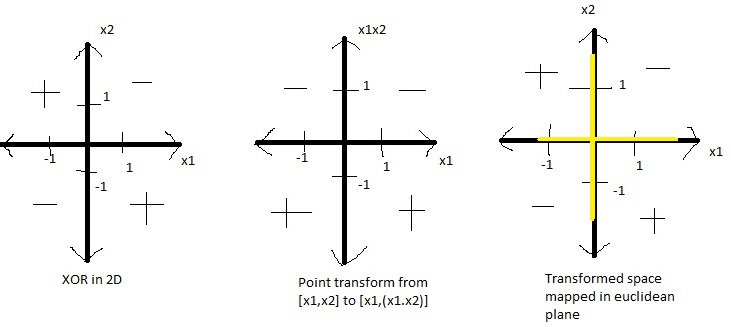
\includegraphics[width=12cm, height=6cm]{ML.jpg}
\end{figure}


\part{2A} For the first required explaination i.e. Dataset1=$\{x_1,x_2,x_3,x_5,x_7\}$.\\
In this case, the linear classifier line having the max margin will run parallely (never meeting) with the line connecting the points $x_1$ and $x_3$, and also the distance of this classifier line equation will be same from both the points $x_1$ and $x_3$ (on 1 part) and having $x_5$ on opposite part. Therefore we can say that, for $D_1$, the max possible margin will be exactly 1/2 length of point $x_5$ from the line which is connecting $x_1$ and $x_3$.\\ The line connecting points $x_1$ and $x_3$ can be observed as Q - P = 0.\\
Here, max margin $D_1$ can be written as:\\
$D_{1}$ = $(1)/(2*\sqrt {2})$\\ 

For the second required explaination i.e. Dataset2=$\{x_1,x_5,x_6,x_8\}$. In this case, the linear classifier line having the max margin will run parallely (never meeting) with the line connecting the points $x_5$ and $x_6$, and also the distance of classifier line equation will be same from both the points $x_5$ and $x_6$ (on 1 part) and having $x_1$ opposite part. Therefore we can say that, for $D_2$, the max possible margin will be exactly 1/2 length of point $x_1$ from the line which is connecting $x_5$ and $x_6$.\\
The line connecting points $x_5$ and $x_6$ can be observed as $\sqrt {3}P + Q - \sqrt {3} = 0$.\\ 
Here, max margin $D_2$ can be written as:\\
$D_{2}$ = $(\sqrt {3})/(4)$ \\ 

For the third required explaination i.e. Dataset3=$\{x_3,x_4,x_5,x_7\}$. In this case, the linear classifier line having the max margin will run parallely (never meeting) with the line connecting the points $x_4$ and $x_3$, and also the distance of classifier line equation will be same from both the points $x_4$ and $x_3$ (on 1 part) and having $x_5$ on the opposite part. Therefore we can say that, for $D_3$, the max possible margin will be exactly 1/2 length of point $x_5$ from the line which is connecting $x_3$ and $x_4$.\\
The line connecting points $x_3$ and $x_4$ can be observed as $2P - Q - 1 = 0$.\\
Here, max margin $D_3$ can be written as:\\
$D_{3}$ = $ (1)/(2*\sqrt {5})$ \\ [15pt]
 
\part{2B}
We know according to perceptron algorithm, mistake bound is given as $<= (R/\gamma)^2$.\\

\bgroup 
\def\arraystretch{1.5}
\begin{tabular}{|l|c|c|c|c|c|} \hline 
{\bf \underline {For D Value}} & {\bf \underline {Most Distant Point}} & {\bf \underline {R}} & {\bf \underline {$\gamma$}} & {\bf \underline {Perceptron Mistake Bound}} \\ \hline
$D_1$ & $x_7$ & 3/2 & $(1)/(2*\sqrt{2})$ & 18 \\ \hline
$D_2$ & $x_8$ & $\sqrt{5}/2$ & $\sqrt{3}/4$ & $6$ \\ \hline
$D_3$ & $x_7$ & 3/2 & $1/(2*\sqrt {5})$ & 45 \\ \hline

\end{tabular}
\egroup

Therefore, $D_3$ has largest mistake bound. \newline


\part{2C}
In terms of ease of learning, the ranking of the given Datasets will be:
$D_2$ $D_1$ $D_3$, where $D_2$ is the easiest to learn.\\
Explaination: As we know that Perceptron Algorithm makes mistakes during learning process, so if lower number of mistakes occur we can tell that the learning of the algorithm did not take place properly, and thus the algorithm's prediction for labels will not be good on the test set. To be more precise, any classifier will learn a bit lower, if the number of mistakes occured during training is lower. Therefore, we can tell that a particular classifier with high mistake bound can behave in a way that is more easy to learn and inversely, smaller mistake bound can behave such that it is harder to learn. This explains the ranking mentioned above.\\

\question{2}{Kernels}

\part{1a} For the requirements above, lets assume some respective gram matrices for a pre-defined space x1,x2,...,xd:
\[ R = \{r_{mn}\}, in-which\{r_{mn}\} equals K_1(x_m, x_n) \] 
\[ S = \{s_{mn}\}, in-which\{s_{mn}\} equals K_2(x_m, x_n) \] \\
The kernel K (product of 2 kernel) can be denoted as:\\
\[K = K_1 X K_2\] \\
Gram Matrix of K will look like:
\[ T = \{t_{mn}\} = \{r_{mn}\}\{s_{mn}\}, in-which \{t_{mn}\}  equals K(x_m, x_n) \]
As we see that the $K_1$ and $K_2$ are symmetric positive definite, so implying this we can say that respective components must be symmetric, that can further expand to:\\ 

    $ R = \{r_{mn}\} = \{r_{nm}\}$, therefore\\ 
$ K_1(x_m, x_n) = K_1(x_n, x_m) $\\
    $ S = \{s_{mn}\} = \{s_{nm}\}$, therefore\\
 $ K_2(x_m, x_n) = K_2(x_n, x_m) $\\

Thus observing the above two equation, we can say that the particular components in the gram matrix for the resultant product kernel will give values as:\\
$ \{t_{nm}\} = \{r_{nm}\}\{s_{nm}\} = \{r_{mn}\}\{s_{mn}\} = \{t_{mn}\}  $\\
Hence, the above product kernel is symmetric, as we can see above.\\
So, as the further step we just need to show that new product kernel is also symmetric positive definite.\\
Lets assume $h \in R^n$ thus we have to represent that $h^TTh >= Zero$.\\ 
    
    $h^TTh = \sum_{mn} h_m h_n t_{mn} = \sum_{mn} h_m h_n r_{mn} s_{mn}$\\

We know by property that any non-singular matrix A can be converted to SPD matrix if it can be multiplied by it's own transpose.\\
Any matrix can be segmented into any matrix and it's transpose.\\
Thus, we will try to segment R and S below:\\ 
    $R = A^TA =$\\ $\{r_{mn}\} = a_{m}^Ta_m = \sum_{k} a_{mk}a_{nk} $\\
    $S = B^TB =$\\ $\{s_{mn}\} = b_{m}^Tb_m = \sum_{l} b_{ml}b_{nl} $\\
   Using these segmented values in above equation, the computation can be extended as:\\
 
    $h^TTh = \sum_{mn} h_m h_n t_{mn} = \sum_{mn} h_m h_n \sum_{k} a_{mk}a_{nk} \sum_{l} b_{ml}b_{nl} =\sum_{kl} \sum_{mn} u_m u_n a_{mk}a_{nk} b_{ml}b_{nl}$\\ 
    $h^TTh = \sum_{kl} \sum_{mn} h_m h_n a_{mk} a_{nk} b_{ml} b_{nl}$\\

As we observe that m and n are independent of each other, so we can segment these as:\\

    $h^TTh = \sum_{kl} ( \sum_{m} h_m a_{mk} b_{ml}) (\sum_{n} h_n a_{nk} b_{nl})$\\
As we observe above, n values are not depending on m, but the values are same, so we can replace any one value:\\    
    $h^TTh = \sum_{kl} ( \sum_{m} h_m a_{mk} b_{ml})^2 >= 0$\\
    Thus we can say that $Gram$ $Matrix$ of T is a SPD.\\
Therefore, it is extablished, K is valid Kernel.\\

\part{1b} 
We will be using the above proved conclusions, to prove the required statement.\\
We need to prove that the addition of kernels and any positive coefficient will be a kernel.\\
According to the requirements, we can establish: \\
$K(x,z) = \alpha K_1(x,z) + \beta K_2(x,z)$\\
where it is given that $K_1(x,z)$, $K_2(x,z)$ = valid kernels.\\
Let us assume $\phi_1$ as a function that maps data vector to feature space of $K_1$, so it can be computed as $K_1(x,z) = \phi_1^T(x)\phi_1(z)$, which can be further written as $<\phi_{1}(x),\phi_{1}(z)>$ denoting the dot product of two vectors\\
Let us assume $\phi_2$ as a function that maps data vector to feature space of $K_2$, so it can be computed as $K_2(x,z) = \phi_2^T(x)\phi_2(z)$, which can be further written as $<\phi_{2}(x),\phi_{2}(z)>$ denoting the dot product of two vectors\\
So using the above equations we can expand as:\\

    $K(x,z) = \alpha K_1(x,z) + \beta K_2(x,z) = <\sqrt[2]{\alpha}\phi_1(x), \sqrt[2]{\alpha}\phi_1(z)> + <\sqrt[2]{\beta}\phi_1(x), \sqrt[2]{\beta}\phi_1(z)>$\\
    $K(x,z) = <[\sqrt[2]{\alpha}\phi_1(x), \sqrt[2]{\beta}\phi_2(x)], [\sqrt[2]{\alpha}\phi_1(z), \sqrt[2]{\beta}\phi_2(z)]>$\\

The above expression proves $K(x,z)$ can be represented as a inner product. Therefore, K is a valid kernel.\\
Now, we see that a polynomial is established by using some positive coefficients. As we saw above sum of two kernels is a kernel and product of a kernel with positive coefficient is a kernel, Therefore K is a valid kernel.\\


\part{2}From the above conclusions we have seen:\\
$K(x,z)$ = $K_{1}(x,z)K_{2}(x,z)$\\
i.e product of two kernel is a kernel\\
Let's start by considering the 2 kernels to be $K_a(x,z) = 15(x^Tz)^2$ and $K_b = \exp(-||x-z||^2)$\\
This implies that if we show that $K_a$ and $K_b$ are indivisual kernels then it can be shown that K is also a valid kernel.\\
Firstly for $K_a$, We will show that $K_a$ is a valid Kernel:\\
We will state the Mercer theorem here:\\
As we know $K_a$ and $K_b$ are kernels, according to mercer's theorem, $K_1$ and $K_2$ should show inner product representation.\\

Lets suppose that $A=p^Tq$ be the required $inner$ $product$ for p and q. We have also concluded above that multiplication of 2 kernel will give a kernel. Thus we can conclude that $A^2 = (p^Tq)(p^Tq) = (p^Tq)^2$ is a valid kernel. Resultant kernel after multiplication with a positive coefficient is also a valid kernel. Here we know, 15 is positive number $\&$ $(p^Tq)^2$ = valid kernel. therefore, we can say that $15(p^Tq)^2$ = valid kernel.\\

Now, as a second case, we need to prove valid kernel condition for $K_b$\\
$K_b$ can further be segmented into:\\
    $K_b(x,z) = \exp(-||x-z||^2)$\\
     = $\exp(-(x-z)^T(x-z))$\\
     = $\exp(-(<x,x-z> - <z,x-z>)) $\\[15pt]
    $K_b(x,z) = \exp(-(<x,x> - <x,z> - <z,x> + <z,z>))$\\
     = $\exp(-(||x||^2 + ||z||^2 - 2<x,z>))$\\[15pt]
    $K_b(x,z) = \exp(-(||x||^2 + ||z||^2)) \exp(2<x,z>)$\\
     = $W\exp(2<x,z>)$\\
    	Here we see that W (any constant) = $\exp(||x||^2 + ||z||^2)$\\
	Then expanding the exponential we get:\\
    $K_b(x,z) = W \sum_{n=0}^\infty \dfrac{<x,z>^n}{n!}$

Therefore, we can observe from the above equation that $K_b$ is created by an $\infty$ addition over polynomial kernels. Also we can observe that these these infinite sum over polynomial kernels, are created using the multiplication of linear kernel $x^Tz$.\\
As we know that sum of valid kernels give valid kernel and product of kernels also give valid kernels, Thus $K_b$ is a valid kernel.\\
As discussed in beginning of proof, K will be a valid kernel as $K_a$ and $K_b$ are valid kernels, as shown above.\\ 

\part{3}
As required in the question, we need to prove that Gaussian kernel can be represented as, inner product of feature space with infinite diamension, which can be represented as:\\
\[K(x,z) = \exp(\dfrac{-||x-z||^2}{2{\sigma}^2})\]

As we have already seen in the above part 1 and part 2 that, the addition of two different kernels can be represented as a kernel:\\
$K(x,z) = K_1(x,z) + K_2(x,z)$\\
We can call the formations for the above equation to be $K(x,z)=\phi$, $K_{1}(x,z)=\phi_1$ and $K_{2}(x,z)=\phi_2$.\\
Thus we observe that $\phi$ is defined in such a way that it can form vector as defined below:\\
$\phi(x) = (\phi_1(x), \phi_2(x))$\\
Using this we may represent the same as we did for poof for addition of kernels:\\
$<\phi(x),\phi(z)> = <\phi_1(x), \phi_1(z)> + <\phi_2(x), \phi_2(z)>$\\
If we extend our discussion to the $Euclidean$ $space$, We may conclude that the vector = $\phi(x)$ is made using segments of $\phi_2$ and $\phi_1$, which further implies:\\[15pt]
$<\phi(x), \phi(z)> = \sum_{i=1}^{dim(K_1)} \phi_{1,i}(x)\phi_{1,i}(z) + \sum_{j=1}^{dim(K_2)} \phi_{1,j}(x)\phi_{1,j}(z)$\\[15pt]
$\implies$ $= \sum_{i=1}^{dim(K_2)+dim(K_2)} \phi_{i}(x)\phi_{j}(z)$\\[10pt]

We can conclude using above statements that, $K_1$ and $K_2$, can be established as infinite sum over kernel polynomials. Therefore $K$ can be mentioned as inner product of a feature space, having infinite diamension as we can observe.\\
In the above proof, K depicts the Radial Basis Function Kernel\\
$K_1$ and $K_2$ depicts the infinite sum Radial Basis Function.\\


\question{3.1}{Experiments - Support Vector Machines}
\part{1}
This has been run on Handwriting dataset.\\
C=1 and $\gamma_{0}$=0.01\\
Weight vector is random ranging from -1 and 1.\\
Bias is also random ranging from -1 and 1.\\
Below results are reported after shuffling the data.\\[15pt]
TEST ON TRAIN SET\\
\bgroup 
\def\arraystretch{1.2}
\begin{tabular}{|l|c|c|c|} \hline 
{\bf \underline {BIAS}} & {\bf \underline {EPOCH}} & {\bf \underline {ACCURACY}} \\ \hline
1 & 3 & 93.1 \\ \hline
-1 & 5 & 92.7 \\ \hline
1 & 8 & 92.9 \\ \hline
1 & 3 & 94.0 \\ \hline
1 & 5 & 93.8 \\ \hline
0 & 8 & 93.7 \\ \hline

\end{tabular}
\egroup\\[20pt]

TEST ON TEST SET\\
\bgroup 
\def\arraystretch{1.2}
\begin{tabular}{|l|c|c|c|} \hline 
{\bf \underline {BIAS}} & {\bf \underline {EPOCH}} & {\bf \underline {ACCURACY}} \\ \hline
-1 & 3 & 91.23 \\ \hline
1 & 5 & 91.06 \\ \hline
-1 & 8 & 91.38 \\ \hline
-1 & 3 & 90.64 \\ \hline
0 & 5 & 90.38 \\ \hline
0 & 8 & 90.05 \\ \hline

\end{tabular}
\egroup

As we see due to random initialization of weight vector and bias and due to shuffling of data, the results vary by a small margin everytime we run the program. The results are however similar for epoch 3 and 5 in every run.

\part{2} 5 - Fold Cross Validation.\\
This has been run on madelon dataset.\\
Weight vector is random ranging from -1 and 1.\\
Bias is also random ranging from -3 and 3.\\
C value used = 0.0312, 0.0625, 0.125, 0.5, 0.25, 1.0\\
$\gamma_{0}$ = 100, 0.1, 0.001, 1\\
Below results are reported after shuffling the data.\\[15pt]
TEST ON TRAIN SET\\
\bgroup 
\def\arraystretch{1.2}
\begin{tabular}{|l|c|c|c|c|c|} \hline 
{\bf \underline {C = Value}} & {\bf \underline {$\gamma_{0}$}} & {\bf \underline {BIAS}} & {\bf \underline {EPOCH}} & {\bf \underline {AVG ACCURACY VALUE}} \\ \hline
0.0312 & 1 & 3 & 3 & 49.75 \\ \hline
0.0312 & 1 & -1 & 3 & 50.08\\ \hline
0.0312 & 1 & 1 & 3 & 51.50\\ \hline
1 & 0.1 & -1 & 3 & 48.09\\ \hline
1 & 0.1 & -1 & 5 & 49.75\\ \hline
1 & 0.1 & -1 & 5 & 49.98\\ \hline
0.5 & 0.01 & -3 & 5 & 53.50 \\ \hline
0.5 & 0.001 & -2 & 8 & 48.00\\ \hline
0.025 & 0.001 & 2 & 8 & 51.50\\ \hline
0.025 & 0.001 & 2 & 8 & 48.09\\ \hline
0.025 & 100 & 1 & 8 & 49.25\\ \hline
0.0625 & 100 & 1 & 5 & 49.98\\ \hline

\end{tabular}
\egroup\\[20pt]


BEST VALUE after running the Cross Validation =\\
C = 0.01\\
$\gamma_{0}$= 0.001\\
Accuracy = 53.50

TEST ON TEST SET\\
\bgroup 
\def\arraystretch{1.2}
\begin{tabular}{|l|c|c|c|c|c|} \hline 
{\bf \underline {C = Value}} & {\bf \underline {$\gamma_{0}$}} & {\bf \underline {BIAS}} & {\bf \underline {EPOCH}} & {\bf \underline {AVG ACCURACY VALUE}} \\ \hline
1 & 1 & 3 & 3 & 49.25 \\ \hline
1 & 1 & -1 & 3 & 50.80\\ \hline
1 & 1 & 1 & 3 & 51.50\\ \hline
0.025 & 0.1 & -1 & 3 & 48.00\\ \hline
0.025 & 0.1 & -1 & 8 & 49.75\\ \hline
0.025 & 0.1 & -1 & 5 & 50.25\\ \hline
0.025 & 0.001 & -3 & 8 & 53.00 \\ \hline
0.025 & 0.001 & -2 & 8 & 53.50\\ \hline
0.5 & 0.001 & 2 & 5 & 51.50\\ \hline
0.5 & 0.01 & 2 & 8 & 52.50\\ \hline
0.5 & 100 & 1 & 8 & 49.25\\ \hline
0.0625 & 100 & 1 & 5 & 50.50\\ \hline

\end{tabular}
\egroup\\[20pt]

BEST VALUE after running the Cross Validation =\\
C = 0.01\\
$\gamma_{0}$= 0.001\\
Accuracy =53.50\\

\part{3}
This has been run on Handwriting dataset.\\
Weight vector is random ranging from -1 and 1.\\
Bias is also random ranging from -3 and 3.\\
Below results are reported after shuffling the data.\\[15pt]
\bgroup 
\def\arraystretch{1.2}
\begin{tabular}{|l|c|c|c|c|c|} \hline 
{\bf \underline {Type}} & {\bf \underline {PRECISION}} & {\bf \underline {RECALL}} & {\bf \underline {F1 - SCORE}} & {\bf \underline {EPOCH}}\\ \hline
TRAIN & 88.94 & 98.35 & 93.41 & 3\\ \hline
TRAIN & 89.40 & 98.54 & 93.75 & 5\\ \hline
TRAIN & 90.08 & 97.81 & 93.78 & 8\\ \hline
TEST & 88.94 & 98.35 & 93.41 & 3\\ \hline
TEST & 89.40 & 98.54 & 93.75 & 5\\ \hline
TEST & 90.08 & 97.81 & 93.78 & 8\\ \hline


\end{tabular}
\egroup\\[20pt]

This has been run on madelon dataset.\\
Weight vector is random ranging from -1 and 1.\\
Bias is also random ranging from -3 and 3.\\
Below results are reported after shuffling the data.\\[15pt]
\bgroup 
\def\arraystretch{1.2}
\begin{tabular}{|l|c|c|c|c|c|} \hline 
{\bf \underline {Type}} & {\bf \underline {PRECISION}} & {\bf \underline {RECALL}} & {\bf \underline {F1 - SCORE}} & {\bf \underline {EPOCH}}\\ \hline
TRAIN & 59.18 & 66.40 & 62.58 & 3\\ \hline
TRAIN & 59.29 & 67.00 & 62.91 & 5\\ \hline
TRAIN & 59.92 & 65.20 & 62.45 & 8\\ \hline
TEST & 64.06 & 54.66 & 58.99 & 3\\ \hline
TEST & 70.77 & 34.66 & 47.81 & 5\\ \hline
TEST & 53.30 & 75.33 & 62.43 & 8\\ \hline

\end{tabular}
\egroup\\[20pt]

\question{3.2}{Experiments - Ensemble of decision trees }
\part{1}
Data run on Handwriting dataset.\\\bgroup
Accuracy of random forest on data\\
 
\def\arraystretch{1.2}
\begin{tabular}{|l|c|c|} \hline 
{\bf \underline {Type}} & {\bf \underline {Accuracy}}\\ \hline
TRAIN & 93.80 \\ \hline
TEST & 89.50 \\ \hline
TRAIN & 93.0 \\ \hline
TEST & 91.00 \\ \hline
TRAIN & 92.00 \\ \hline
TEST & 91.21 \\ \hline
TRAIN & 89.23 \\ \hline
TEST & 88.22 \\ \hline

\end{tabular}
\egroup\\[20pt]




\end{document}